\documentclass[a4paper,12pt]{scrartcl}
\usepackage{enumerate}
\usepackage{graphicx}
\usepackage[none]{hyphenat}
\usepackage{tikz}
\usepackage{amsmath}
\usepackage{pgfplots}
\usepackage{booktabs}
\usepackage{caption}
\usepackage{array} 
\usepackage{braket}
\usepackage[section]{placeins}

\usetikzlibrary{shapes}
\usetikzlibrary{arrows}
\usetikzlibrary{calc,positioning}
\pgfplotsset{compat=1.9} 


\newcommand\independent{\protect\mathpalette{\protect\independenT}{\perp}}
\def\independenT#1#2{\mathrel{\rlap{$#1#2$}\mkern2mu{#1#2}}}

\begin{document}
\title{Graphical Models}
\subtitle{Data Mining 2015: assignment 2}
\author{Sebastiaan Jong (5546303) \& Bas Geerts (5568978)}
\date{}
\maketitle
\section{Data Analysis}
Questions:
	\begin{enumerate}[(a)]
		\item The data contains 10 columns, hence we have 10 nodes. Every possible configuration of edges between these 10 nodes is a graphical model. Looking at an 10 by 10 adjacency matrix, it is clear that $9 + 8 + 7 + \dots + 2 + 1 = 45$ variables are required to define the graph. We can ignore most positions in the matrix, since it is symmetric and because nodes can not have edges to themselves. Over 45 binary variables there are $2^{45}$ different configurations. 
		\item The amount of parameters in a saturated model are is equal to the amount of cells in the table of counts, since we make no independence assumptions. The amount of cells in the table of counts is equal to the product over all possibilities per variable. For this dataset, that is $7 \cdot 2 \cdot 2 \cdot 2 \cdot 3 \cdot 6 \cdot 4 \cdot 3 \cdot 5 \cdot 2 = 155520$ cells.
		\item Performing a forward-backward search with the BIC score function on this data starting from the empty graph gives us a model with a score of 15841.66 and 13 cliques. The cliques are listed in Table \ref{tab:c}. The graphical model is shown in Figure \ref{fig:c}.

		    \begin{table}[!htb]
			    \small  
		        \centering
		        $\begin{array}{ *{5}{c} }
		            \midrule
		                  \set{1,8}  & \set{1,9}  & \set{2,8} &  \set{2,9} &  \set{2,10} \\
		                  \set{3,6}  & \set{4,6}  & \set{5,6} &  \set{5,10} &  \set{6,7} \\
		                  \set{6,8}  & \set{6,9}  & \set{1,3,10} \\
		            \bottomrule
		        \end{array}$
		        \caption{Cliques found in (c).}
		        \label{tab:c}
			\end{table}
			\begin{figure}
				\centering
				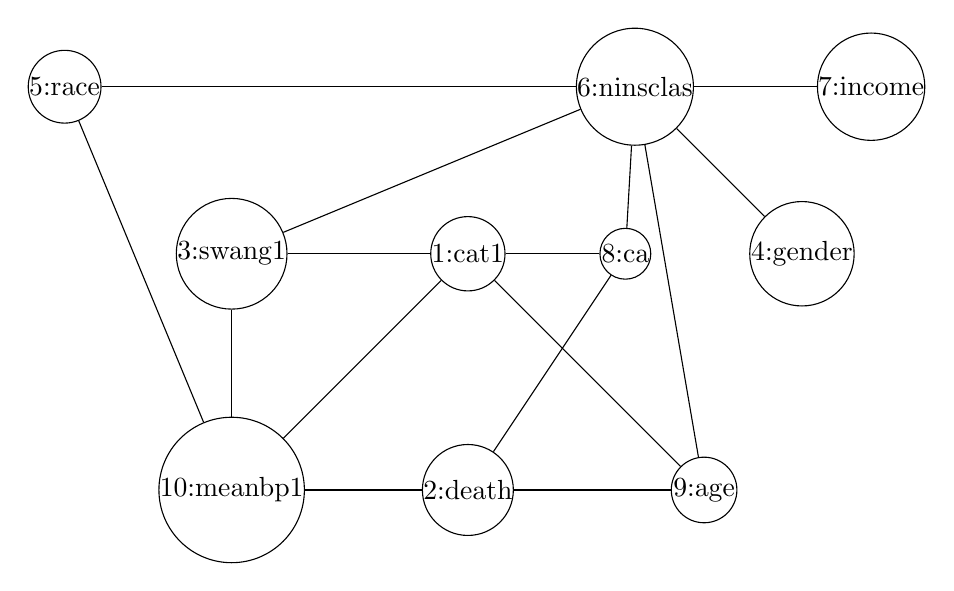
\begin{tikzpicture}[ball/.style = {circle, draw, align=center, inner sep=0}, node distance=3cm]

\node[ball](1){1:cat1};
\node[ball, left of =1](3){3:swang1};
\node[ball, below of=3](10){10:meanbp1};
\node[ball, right of=10](2){2:death};
\node[ball, right of=2](9){9:age};
\node[ball, right of=1, node distance=2cm](8){8:ca};
\node[ball, above right of=1](6){6:ninsclas};
\node[ball, right of=6](7){7:income};
\node[ball, above left of=3](5){5:race};
\node[ball, below right of=6](4){4:gender};

\draw [-] (1) to (3);
\draw [-] (1) to (10);
\draw [-] (3) to (10);
\draw [-] (1) to (8);
\draw [-] (3) to (6);
\draw [-] (6) to (8);
\draw [-] (1) to (9);
\draw [-] (2) to (8);
\draw [-] (2) to (9);
\draw [-] (4) to (6);
\draw [-] (6) to (9);
\draw [-] (5) to (6);
\draw [-] (5) to (10);
\draw [-] (6) to (7);
\draw [-] (2) to (10);



\end{tikzpicture}
				\caption{Independence graph found in (c).}
				\label{fig:c}
			\end{figure}
		\item Based on the independence graph found in (c), we can state that $income \independent gender\ |\ ninsclass$. To predict whether someone survives, we need the variables \textit{ca}, \textit{age} and \textit{meansbp1}. The variable \textit{death} has no edges to other nodes, so it is independent of the rest of the graph when these three variables are given. 
		\item  Performing a forward-backward search with the BIC score function on this data starting from the complete graph gives us a model with a score of 15850.53 and 15 cliques. The cliques are listed in Table \ref{tab:e}. The graphical model is shown in Figure \ref{fig:e}. One of the major differences of this graph compared to the one from (c) is that both income and now both have more than one edge. The score of these models is nearly the same. 
		    \begin{table}[!htb]
			    \small  
		        \centering
		        $\begin{array}{ *{5}{c} }
		            \midrule
  						\set{1,8} & \set{1,3,10} & \set{2,7} & \set{2,8} & \set{2,9} \\
  						\set{2,10} & \set{3,4} & \set{3,9} & \set{4,6} & \set{5,7} \\
  						\set{5,9} & \set{5,10} & \set{6,7} & \set{6,8} & \set{6,9} \\ 
		            \bottomrule
		        \end{array}$
		        \caption{Cliques found in (e).}
		        \label{tab:e}
			\end{table}
			\begin{figure}
				\centering
				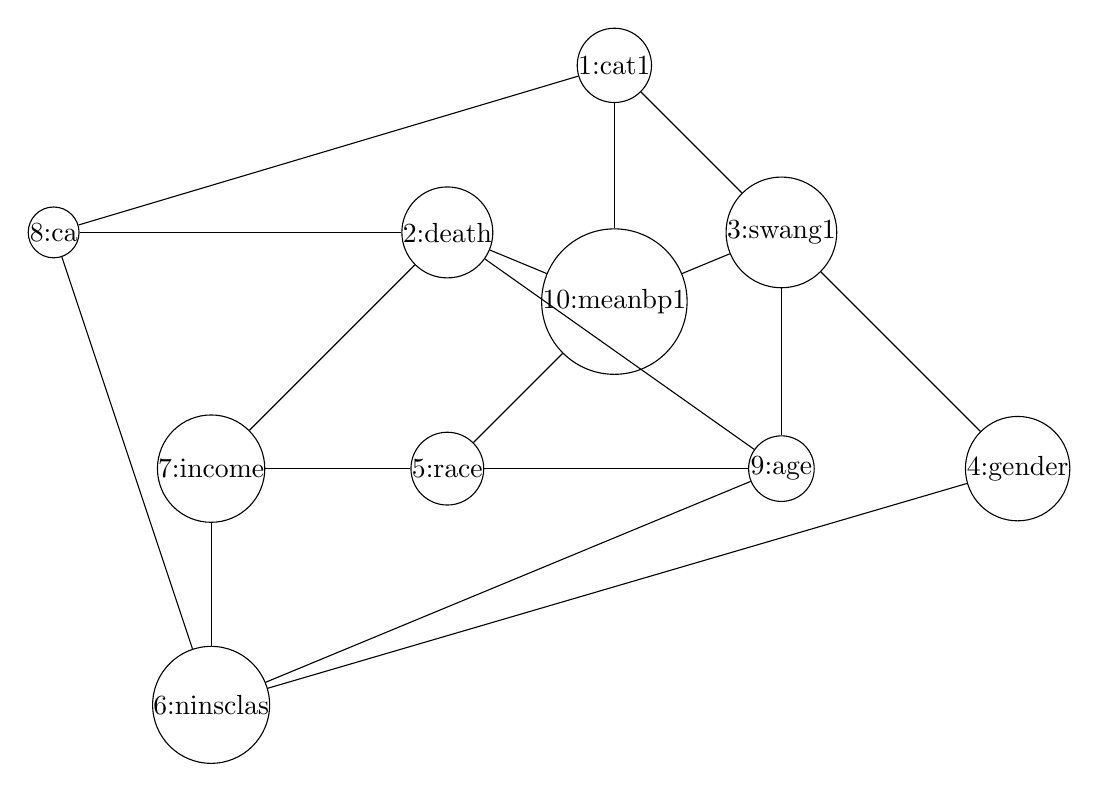
\begin{tikzpicture}[ball/.style = {circle, draw, align=center, inner sep=0}, node distance=3cm]

\node[ball](1){1:cat1};
\node[ball, below right of=1](3){3:swang1};
\node[ball, below of=1](10){10:meanbp1};
\node[ball, below left of=1](2){2:death};
\node[ball, below right of=10](9){9:age};
\node[ball, below left of=10](5){5:race};

\node[ball, left of=5](7){7:income};

\node[ball, below of=7](6){6:ninsclas};
\node[ball, right of=9](4){4:gender};
\node[ball, left of =2,node distance=5cm](8){8:ca};

\draw [-] (1) to (8);
\draw [-] (1) to (3);
\draw [-] (1) to (10);
\draw [-] (10) to (3);
\draw [-] (2) to (7);
\draw [-] (2) to (8);
\draw [-] (2) to (9);
\draw [-] (2) to (10);
\draw [-] (4) to (3);
\draw [-] (9) to (3);
\draw [-] (4) to (6);
\draw [-] (5) to (7);
\draw [-] (5) to (9);
\draw [-] (5) to (10);
\draw [-] (6) to (7);
\draw [-] (6) to (8);
\draw [-] (6) to (9);



\end{tikzpicture}

				\caption{Independence graph found in (e).}
		        \label{fig:e}
			\end{figure}
		\item Starting the local search with an empty graph and using the AIC scoring function a local optimum of 14278.21 was found by the algorithm. The 14 cliques for this search can be seen in Table \ref{tab:f}. Using the complete graph, exactly the same score and cliques were found.
		    \begin{table}[!htb]
			    \small  
		        \centering
		        $\begin{array}{ *{5}{c} }
		            \midrule
						\set{4,5,6} & \set{4,6,8} & \set{1,4,8} & \set{1,4,10} & \set{4,5,10} \\
						\set{2,7} & \set{5,6,7} & \set{1,2,8} & \set{1,2,9} & \set{1,3,9} \\
						 \set{3,6,9} & \set{5,6,9} & \set{1,2,10} & \set{1,3,10} \\ 
		            \bottomrule
		        \end{array}$
		        \caption{Cliques found in (f) while searching from an empty graph.}
		        \label{tab:f}
			\end{table}

		\item The BIC scoring function penalizes large models more severely than AIC. This also can be seen in the results obtained in (f) compared to (c) and (e). In (e), we found several cliques of size 3, since the AIC function is more willing to add additional edges. Cliques found in (f) and (c) mainly are of size 2. 
		\item 
	\end{enumerate}
\end{document}


